% ===========================================================
% 1. INTRODUCTION
% ===========================================================
\section{Introduction}
\label{sec:intro}

Embodied navigation serves as a fundamental capability for general-purpose physical agents, bridging high-level cognition and low-level motor control~\cite{anderson2018vln,gu2022vlnsurvey,hossain2026review,yang2025nav,gong2026poinavbenchmarkingenhancingfinalmeters,yang2026asyncshieldplugandplayedgeadapter,chen2026explorelikehumansautonomous,chu2026abotn0technicalreportvla,chen2026astranavworldworldmodelforesight,xiang2025navr2dualrelationreasoninggeneralizable,Liu_2026_CVPR,Chen_2026_CVPR,xue2026omninavunifiedframeworkprospective,yang2025cenavflowguidedreinforcementrefinement}. 
A truly versatile navigator must operate in open-world environments—where lighting, geometry, dynamics, and social norms vary continuously—to reach precise metric targets, follow free-form natural-language instructions, search for open-vocabulary objects, locate points of interest (POIs), and track moving people.
However, historically, these abilities have been pursued in isolation. 
Tasks such as \textit{point-goal}, \textit{object-goal}, \textit{POI-goal}, \textit{instruction-following}, and \textit{person-following} are typically dominated by task-specific architectures characterized by bespoke goal interfaces, narrow training data, and limited cross-task transfer~\cite{anderson2018vln,batra2020objectnav,krantz2020vlnce,savva2019habitat}.
This fragmentation hinders the extraction of physical and semantic priors from heterogeneous data, resulting in a ``\textit{zoo}'' of specialized models that are difficult to integrate into a single robot.


Recent efforts address this fragmentation by developing general-purpose navigation foundation models~\cite{zhang2025navfom,abotn0,sun2026openfrontier,chen2025socialnav} that unify diverse tasks within a single architecture and corpus. 
While this paradigm has demonstrated improved cross-task transfer, three critical \textbf{challenges} persist as these generalist models transition from benchmark leaderboards to real-world robotic deployment:
\begin{itemize}

\item \textbf{To-Point Navigation.} Target coordinates are specified as ego-centric offsets relative to the robot’s pose. However, inaccuracies in Standard-Definition (SD) map routing or localization can shift these targets into physically infeasible regions—such as vehicle lanes or flower beds—instead of valid walkable paths. This misalignment necessitates explicit traversability reasoning to ensure safe arrival.

%\item \textbf{To-Target Navigation:} Current approaches often rely on rigid semantic representations, such as fixed category embeddings or single-text-token proxies, which lack the granularity to capture nuanced visual-linguistic alignments. Consequently, these models tend to fail silently when encountering long-tail instances or compositional queries;

\item \textbf{To-Target Navigation.} End-to-end fine-tuning on object-search trajectories risks eroding pretrained semantic priors critical for open-vocabulary recognition. Moreover, conflating ``search'' and ``approach'' phases couples stochastic exploration with deterministic execution, leading to brittle training convergence and ambiguous failure attribution.

\item \textbf{Interpretability \& Safety.} Monolithic policies that map observations directly to actions operate as black-box systems, lacking explicit, human-readable decision traces or intermediate reasoning steps. This opacity obscures the causal link between sensory inputs and motor outputs, severely hindering root-cause analysis of failures and complicating safety audits, as developers cannot easily discern whether errors stem from perception, reasoning, or control modules.
\end{itemize}

% entanglement of exploration and reaching
%For example, \textit{object-goal} navigation, where end-to-end fine-tuning on object-search trajectories can erode the pretrained semantic priors essential for open-vocabulary recognition. Furthermore, conflating “find the object” and “reach the object” into a single trajectory entangles open-ended exploration with final-approach execution, making training convergence brittle and per-episode failures difficult to attribute to either phase.

%pathologies are most visible on \textit{object-goal} navigation, where end-to-end fine-tuning of a single policy on object-search trajectories erodes the very pretrained semantic priors that open-vocabulary recognition relies on, and where packing both ``find the object'' and ``reach the object'' into one trajectory entangles open-ended exploration with final-approach execution---making training convergence brittle and per-episode failures hard to attribute to either phase.


These pain points share a fundamental architectural root cause: the reliance on monolithic policies that bypass intermediate reasoning. 
This design suffers from two critical flaws. 
Firstly, it creates a spectral mismatch between the slow dynamics of semantic reasoning and the fast dynamics of motor control, forcing distinct computational processes into a single update cycle. 
Secondly, optimizing for heterogeneous tasks within a shared parameter space leads to optimization interference, where conflicting gradients from diverse objectives (e.g., precision navigation vs. semantic exploration) cause negative transfer~\cite{yu2020gradient,liu2021conflict}. 
We argue that a modular, factorized approach offers a superior solution. 
By decoupling cognition from control, we enable a low-frequency reasoner to perform explicit planning and a high-frequency controller to handle reactive execution. These components interact through a transparent, structured bottleneck, replacing the black-box latent representations of traditional end-to-end models.


Motivated by these insights, we introduce \textbf{ABot-N1} (see Figure~\ref{fig:overview}), a Vision-Language-Navigation (VLN) foundation model featuring a hierarchical \textbf{slow–fast} architecture. The slow subsystem employs a 4B-parameter multimodal VLM to conduct high-level deliberative reasoning. By processing instructions, visual memory, and current observations, it produces a CoT rationale that interprets intent, grounds language to visual entities, and adheres to social norms ~\cite{wei2022cot,deepseekai2025r1,chen2025socialnav}. Crucially, this reasoning process yields a pixel goal—a compact set of 2D anchors in the egocentric view that defines the next sub-goal. The fast subsystem, a specialized 2B-parameter VLM, acts as a low-latency action expert. It synthesizes the slow system’s CoT and pixel goal with real-time visual inputs to emit continuous waypoints, ensuring responsive control at the robot’s native frequency.

The core design principle of our architecture lies in its \textbf{dual-modality guidance}: the slow system emits a CoT for semantic reasoning and a Pixel Goal for spatial grounding. 
The linguistic traces provide robust, transferable high-level logic, while the pixel goal translates this logic into actionable, egocentric visual anchors. 
Regardless of the initial task formulation---whether a metric coordinate, a free-form instruction, an object category, a POI name, or a target person---it is decomposed into this shared language-plus-vision representation.
By reducing all tasks to \textit{``tracking CoT-explained pixels''}, the fast controller operates on a consistent interface regardless of input complexity. 
This approach generalizes earlier visual-prompting techniques~\cite{feng2026vpn,nasiriany2024pivot,sun2026openfrontier} by evolving from passive, user-defined prompts to active, reasoning-aware model generations. 
As a result, the framework seamlessly handles geometric, semantic, and dynamic targets. 
Three distinct \textbf{advantages} emerge from this design:
\begin{itemize}

\item \textbf{To-Point Navigation.} By performing image-space re-grounding at each step, we mitigate the sensitivity to coordinate inaccuracies inherent in ego-centric offset targets. When localization or map errors shift the goal into non-traversable areas, the CoT-guided affordance pixels automatically correct the trajectory toward the nearest safe pathway, preventing the agent from getting stranded in prohibited regions—a common failure mode for metric-only baselines.

\item \textbf{To-Target Navigation.} By offloading open-vocabulary recognition to the deliberative slow reasoner, we decouple semantic understanding from reactive control. The slow system utilizes its robust pre-trained priors to resolve ambiguities in long-tail distributions and compositional queries, which are typically prone to failure in end-to-end policies. This separation ensures that complex semantic interpretations do not compromise the stability of the fast controller, leading to more reliable identification of novel and intricate targets.

\item \textbf{Interpretability \& Safety.} By integrating human-readable CoT reasoning with visually grounded pixel anchors, our architecture achieves fine-grained interpretability at every decision step. This transparency is crucial for safety-critical applications, as it allows for precise root-cause analysis of failures. Developers can distinguish whether an error stems from flawed semantic reasoning (visible in the CoT) or inaccurate spatial targeting (visible in the pixel goal), thereby accelerating debugging and ensuring that the robot’s behavior aligns with human expectations and safety constraints.
\end{itemize}

\begin{figure}[t]
\centering
% 
\includegraphics[width=\linewidth]{figs/overview.pdf}
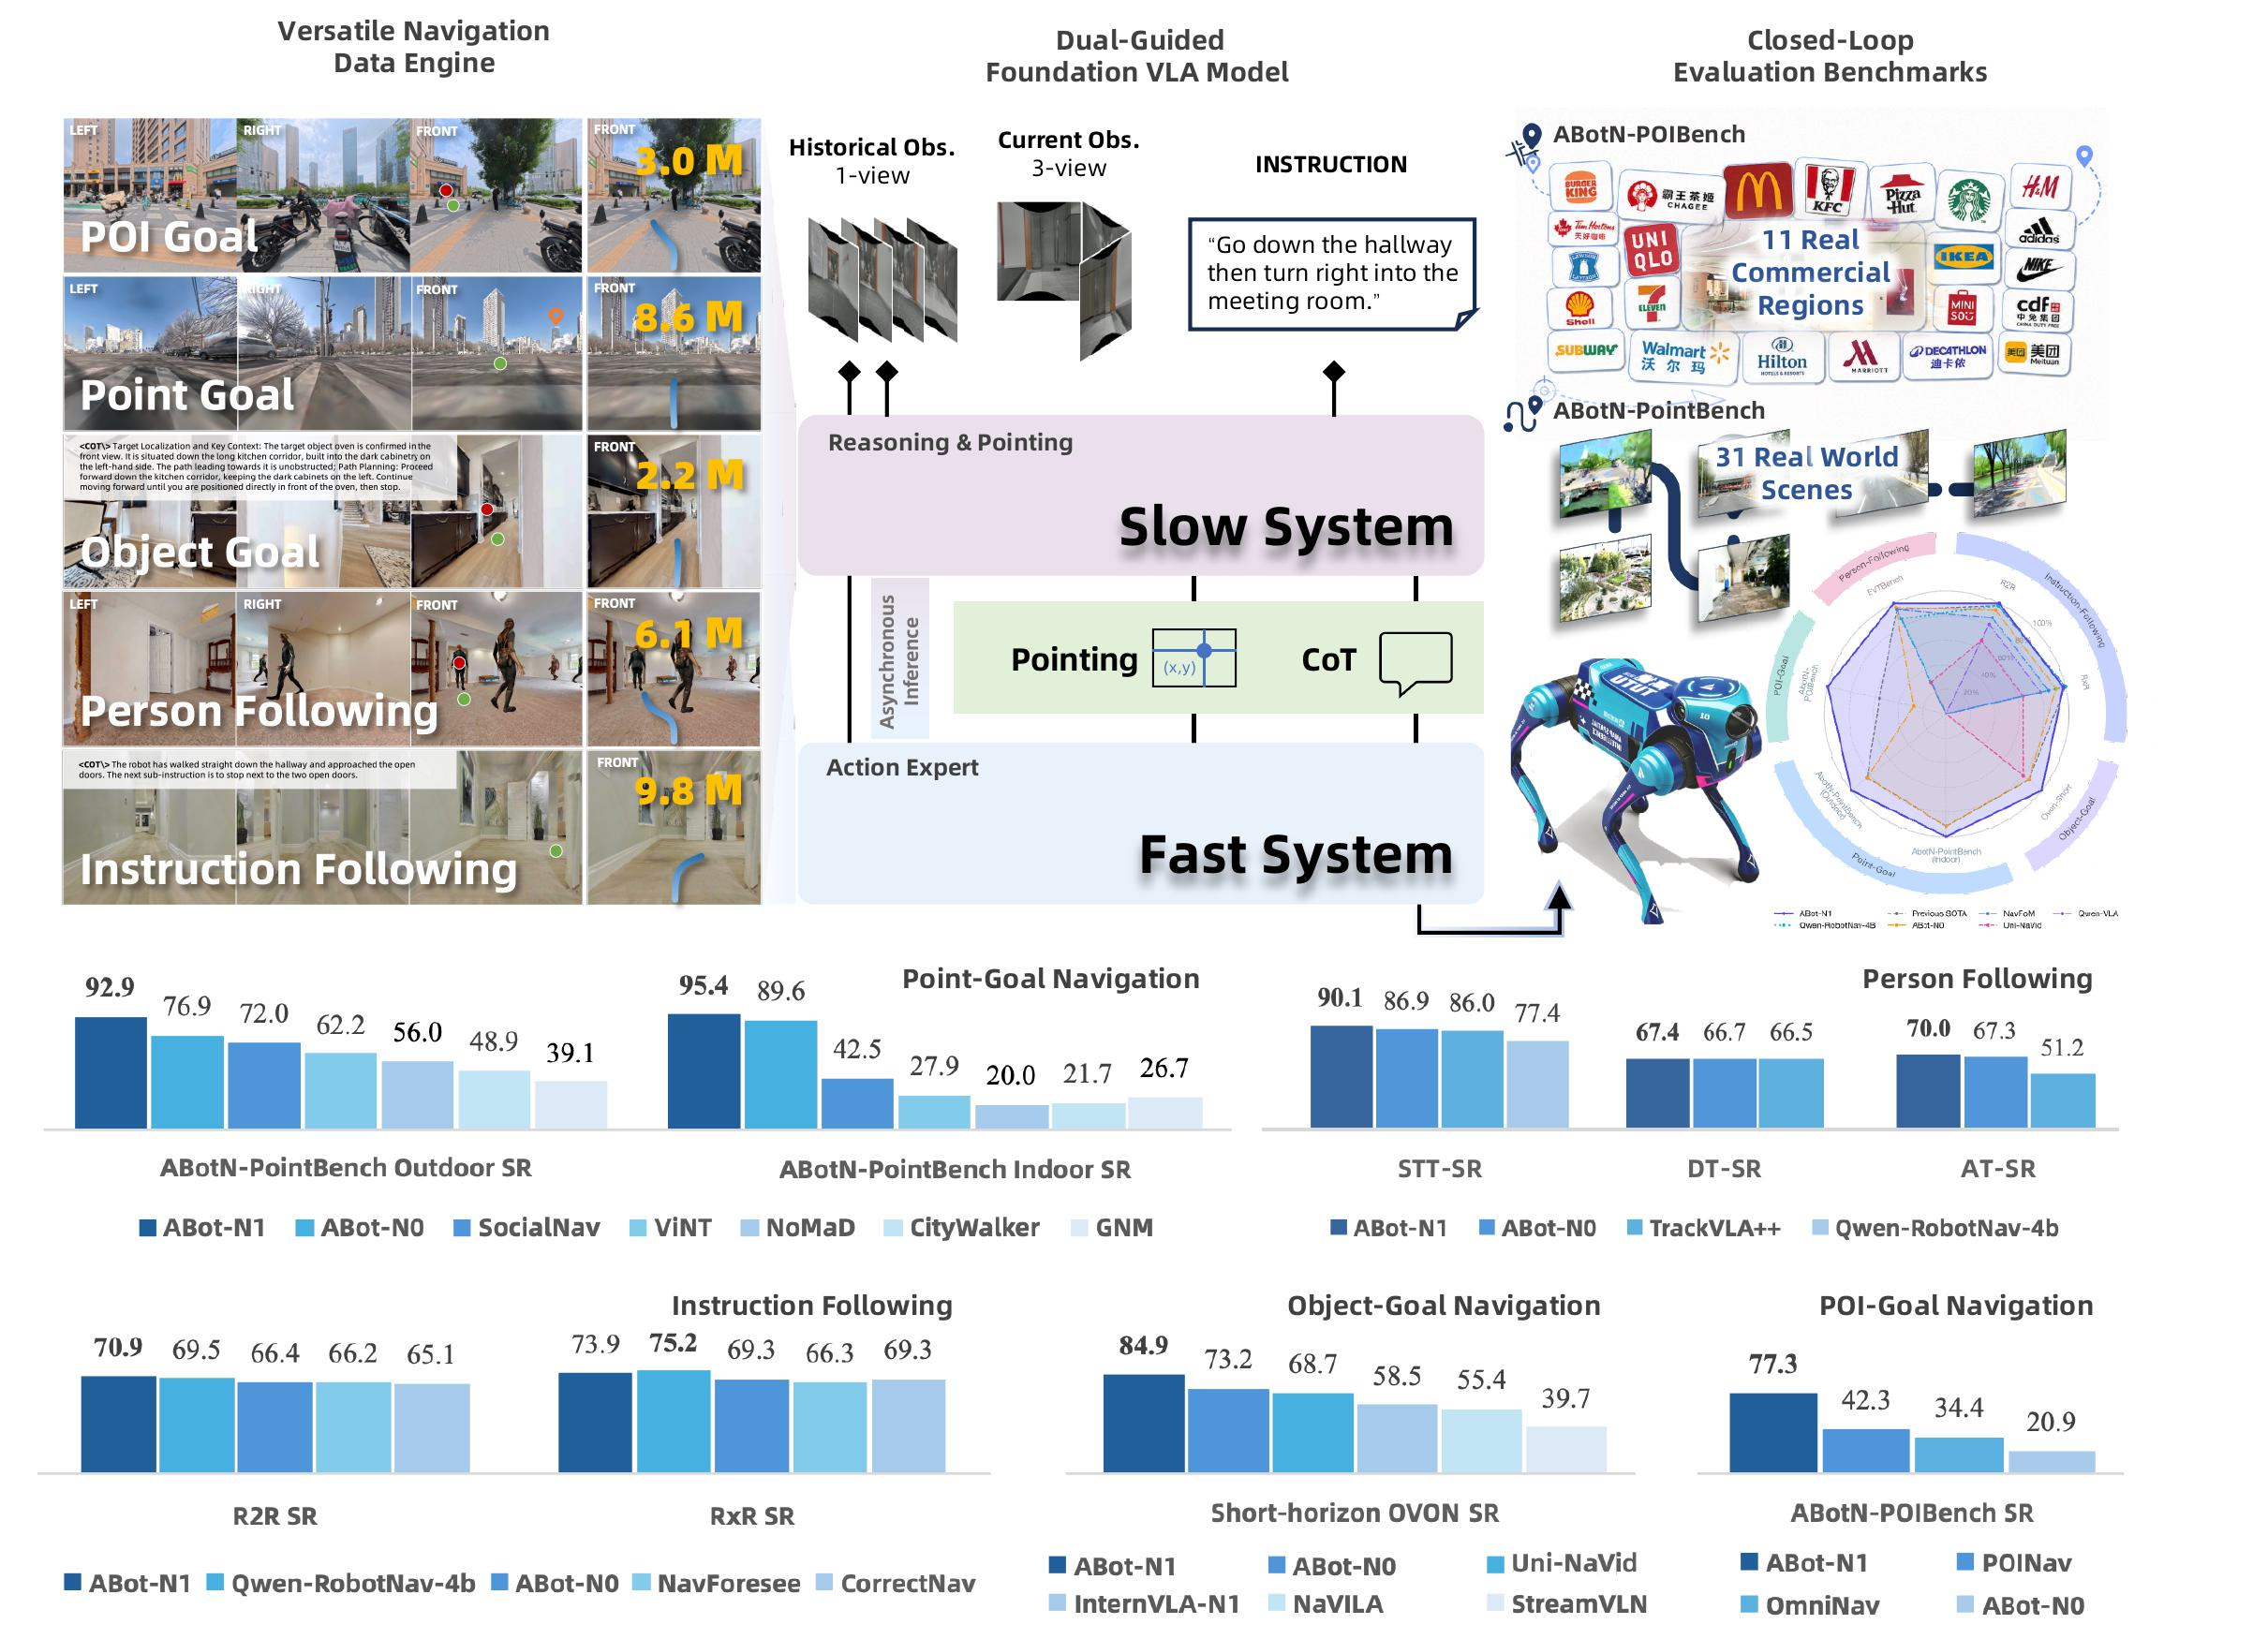
\includegraphics[width=\linewidth]{figs_jpg/overview.jpg}

\caption{\textbf{Overview of ABot-N1.} The model trained on 30M samples across five tasks adopts a slow--fast control architecture: a slow system performs CoT reasoning and emits pixel goals, while a fast action expert consumes this dual language-and-vision guidance to execute safe waypoints.
Closed-loop evaluation is conducted on our newly proposed ABotN-PointBench and ABotN-POIBench, together with three established benchmarks (VLN-CE R2R/RxR, Short-Horizon OVON, and EVT-Bench). ABot-N1 achieves leading performance across all 5 benchmarks.}
\label{fig:overview}
\end{figure}

Realizing this design at scale requires overcoming the data and optimization bottlenecks prevalent in existing generalist models. We address this by extending our prior data infrastructure~\cite{abotn0} with high-fidelity, pixel-grounded reasoning traces for all target tasks. Crucially, we depart from standard token-level supervision by introducing a GRPO-based reinforcement learning stage~\cite{deepseekai2025r1} for the slow system. This mechanism aligns the model’s output with actual task completion rather than just linguistic plausibility, thereby enhancing the robustness and physical feasibility of the generated pixel goals.


Despite the maturity of benchmarks for \textit{instruction-following} and \textit{object-goal} tasks~\cite{anderson2018vln,ku2020rxr,krantz2020vlnce,yokoyama2024hmovon}, open-source evaluation frameworks for cityscale navigation—specifically \textit{point-goal} and \textit{POI-goal}—remain notably scarce. 
We bridge this gap by releasing two novel benchmarks: \textbf{ABotN-PointBench} covering complex indoor and outdoor environments, and \textbf{ABotN-POIBench} situated in realistic commercial districts. 
Through a hierarchical difficulty structure, these benchmarks enable comprehensive assessment of state-of-the-art methods and demonstrate the superior capabilities of ABot-N1. 
We make both benchmarks publicly available to foster further advancements in the field.
%Realizing this design at scale also requires data and benchmarks beyond what current generalist navigators rely on. We extend our previous data engine~\cite{abotn0} with pixel-grounded trajectories and reasoning samples for all five tasks, and introduce a post-training stage that applies GRPO-style reinforcement learning~\cite{deepseekai2025r1} to the slow system in order to align its pixel generation with downstream navigation success rather than merely with token-level supervision. While \textit{instruction-following} and \textit{object-goal} already enjoy mature benchmarks~\cite{anderson2018vln,ku2020rxr,krantz2020vlnce,yokoyama2024hmovon}, open-source benchmarks for \textit{point-goal} and \textit{POI-goal} evaluation remain extremely scarce. We therefore release a new Point-Goal Benchmark spanning indoor and outdoor scenes, together with a POI-Goal Benchmark grounded in real commercial districts; through a multi-level difficulty design, both benchmarks comprehensively evaluate representative prior methods as well as the performance gains delivered by ABot-N1, and are released as open source.

\textbf{In summary, this report makes the following contributions:}
\begin{itemize}
  \item \textbf{Architecture.} We introduce ABot-N1, a dual-system VLA navigator featuring a slow–fast architecture and a unified pixel-goal interface. It provides joint semantic-spatial guidance via CoT and image anchors for five key tasks: \textit{point-goal}, \textit{object-goal}, \textit{POI-goal}, \textit{instruction-following}, and \textit{person-following}.
  
  \item \textbf{Training Recipe.} Building on the ABot-N0 data engine~\cite{abotn0}, we integrate pixel-grounded supervision and CoT trajectories for all five tasks. Furthermore, we employ GRPO-style post-training~\cite{deepseekai2025r1} to align the slow system's reasoning directly with downstream navigation rewards.
  
  \item \textbf{Cityscale Benchmarks.} We release ABotN-PointBench and ABotN-POIBench, which comprehensively evaluate \textit{point-goal} navigation (short/long-range, indoor/outdoor) and \textit{POI-goal} navigation in real-world commercial scenarios.
  
  \item \textbf{Cityscale Navigation.} Using a unified checkpoint, ABot-N1 achieves state-of-the-art performance across five tasks, exceeding both specialized and multitask models. It further propels urban navigation forward by enabling robust long-horizon autonomy in complex cityscapes with only low-fidelity SD maps, thereby overcoming the traditional reliance on high-precision infrastructure.
  
\end{itemize}

More intuitively, this slow-fast separation allows us to treat semantic recognition and motor action as distinct data streams. By decoupling the slow reasoning system from the fast control system, we effectively disentangle these domains—a distinction crucial for open-world scaling as it enables the independent expansion of training corpora for perception and control without interference. Having already validated the effectiveness of this paradigm in \textbf{ABot-N1}, we plan to further verify the efficacy of this data-centric scaling strategy in our next iteration, \textbf{ABot-N1.1}.